
\subsection{A crowdsourced historical reading comprehension task}
We designed a crowdsourced historical reading comprehension task to compare \ours~with a \Baselongname~system (IR),
 which we consider to be a baseline tool for historical research (Section \ref{s:intro} and \ref{s:related}).
Our task is designed to reflect historians' common practice of mention gathering and analysis, in which expert social researchers find and review occurrences of a query $Q$ in an archive (Section \ref{s:intro}) in order
to draw conclusions about society.
In our crowdsourced adaptation of this common historical research process, we tasked non-specialists with finding and reviewing occurrences of a query in a newspaper corpus.\footnote{We did not ask participants to take the next step of drawing substantive historical conclusions from their findings, which would have required deep historical knowledge and specialized training.}
We then used reading comprehension questions to measure how well participants performed at finding and reviewing information about the query;
many common educational assessments use similar reading comprehension questions to assess how well people learn information from documents \cite[Chp.\ 7]{reading_comp}.

To ensure we presented an ecologically-valid research prompt, we modeled our crowd task after a real historical question from P2. 
In our interview study (Section \ref{s:usabilitystudy}), P2 used \ours~to investigate if \textit{The New York Times} portrayed the controversial figure Robert Mugabe as a corrupt authoritarian, or as a hero of Zimbabwe's fight for independence. 
In our crowd study, we presented participants with one of two text analytics tools loaded with the same small corpus of 12 \textit{New York Times} editorials mentioning Robert Mugabe, published from January, 2001 to June, 2003. 
We then asked participants to ``find and remember everything the \textit{The New York Times} wrote about Robert Mugabe'' using their tool.
Because historians have only so much time for a given research project (Section \ref{s:needs_comprehensive}), we limited participants to exactly six minutes to conduct their research using their assigned interface. After six minutes, we presented eight true/false reading comprehension questions about \textit{New York Times} coverage of Mugabe, and observed the total number of correct answers for each participant.
Because scoring well on this test of reading comprehension requires finding and reviewing information about a query in a corpus, we believe our crowd task measures how well people perform mention gathering and analysis, using a particular interface.

\subsubsection{Details: reading comprehension questions and scoring}

In order to ensure that our task was as objective and neutral as possible, we created reading questions using the Wikipedia page for Robert Mugabe \cite{wikimugabe}.
Specifically, we used a semi-automated procedure based on tf-idf sentence vectors (described in detail in the Appendix) to identify Mugabe facts from Wikipedia reported in \textit{New York Times} editorials about Mugabe.
We then selected four facts from Wikipedia reported in the 12 editorials in the corpus, and four facts from Wikipedia that were not reported in the 12 editorials. These four facts were reported in some other \textit{New York Times} editorial that was not presented to participants (because the editorial was published before or after January, 2001 to June, 2003). In total, this process created a list of eight total Mugabe facts from Wikipedia.


To evaluate reading comprehension, we presented all eight facts in randomized order, and asked participants to select those facts which appeared in the articles they had reviewed during the task.
To get a perfect score of eight out of eight correct answers without guessing,\footnote{In this task, a participant would have a $.5^8 * 100 = 0.391\%$ chance of correctly guessing all 8 answers.} a participant would have to find and remember the four Mugabe facts reported in the editorials shown during the task, without selecting any of the four facts that were not reported in the editorials. 
The Appendix includes a screenshot showing the reading comprehension questions.


\subsection{Experiment design and experiment details}

We compared \ours~with a \Baselongname~system using a between-subjects experiment design with U.S.\ masters workers recruited via Amazon Mechanical Turk. (Amazon confers the master designation on crowdworkers with a record of success in crowd tasks.)
Participants were randomly assigned to complete the reading comprehension task using either \ours~or a baseline \Baselongname~interface (IR). We then measured the difference in the mean number of total correct answers from workers in each group to determine if \ours~helped people find and remember information about Robert Mugabe (as compared to the IR system).

\subsubsection{Implementation of the IR baseline}
We implemented the IR system using Whoosh, an open-source Python \Baselongname~tool which ranks results using the common BM25 metric.\footnote{Whoosh is similar to other traditional \Baselongname~tools like Lucene. \url{https://whoosh.readthedocs.io/}} The Appendix contains a screenshot of this baseline interface.

To ensure fair comparison, we tuned Whoosh to be most similar to \ours.
Specifically, Whoosh accepts a number of configuration parameters which govern how the system creates snippets on the results page (see Section \ref{s:related_work_search}). 
Because such snippets are similar to the snippets in the \ours~Document Feed, we adjusted the Whoosh snippet parameters so that that Whoosh snippets were as close as possible in length to the shortened sentences in the \ours~Document Feed.
Further details about the tuning procedure are described in the Appendix.
We also adjusted the IR system to use the same font size as \ours.

To minimize possible variation in worker behavior, we hard-coded the IR system (and the \ours~system) to use the query ``Mugabe'' during the experiment.\footnote{During the experiment, we also removed \ours~interface elements which are not relevant for the task, such as the corpus selection control, filter-by-date feature and filter-by-subquery feature.}
To rank the 12 documents in the corpus using the IR system, we loaded the IR tool with all \textit{New York Times} editorials published between 1987 and 2007 that include the word ``Zimbabwe,'' and then queried for ``Mugabe'' while applying a date filter to select only those results which were published from January, 2001 to June, 2003.

We did not implement the IR system using proprietary black-box search tools like Google or \textit{New York Times} search \cite{nytwebsite}.
This is because it is not possible to load open-source versions of such systems with a custom corpus.
Loading a custom corpus is crucial for two reasons. 
(1) Our broader goal is to design an open-source software system that can be deployed and used by historians, who are often interested in corpora that are not published on the web (Section \ref{s:limits_and_future}) and thus inaccessible to Google (or to any other web search engine product).
Comparing to an open-source search engine is thus more appropriate than comparing to a black-box system like Google. 
A historian could use an open-source search engine to index and analyze the documents they collect during their work.
(2) For a controlled experimental comparison of two user interfaces, it's necessary to fix the dataset used for both interfaces. 
In our experiment, users were evaluated based on what information they found (which would change based on the dataset).

\subsubsection{Experiment sequence, experiment pretest, and phases of data collection}

At the start of the experiment, participants in each condition watched a roughly one minute training video describing how to use their randomly assigned interface.
They also read several screens with task instructions, where they entered short phrases into text boxes to confirm they understood the task and were paying attention.
After these preliminaries, participants took an easy pretest which was very similar to the main task (but was about Iraq instead of Zimbabwe).
We describe the details of the pretest in the Appendix.
After the pretest, participants proceeded to the main Robert Mugabe task, conducted their research, and answered the eight reading comprehension questions.
The task concluded with qualitative questions, including questions about the strengths or weaknesses of the assigned interface. 
Qualitative questions are provided in the Appendix.
In total, the task took 20 minutes.

Data collection for the task proceeded in two phases. We first collected data from 18 participants in a small initial pilot. Following the initial pilot, we made adjustments to the task described in the Appendix, including fixing a bug which was favorable to the IR baseline. Following these changes, we collected data from the remaining 103 participants. We decided to include data from the pilot in our analysis because collecting data from crowdworkers was expensive, and because we had trouble recruiting participants from the limited pool of masters workers. (Pooling data is common in settings where data is sparse).
Because we struggled with recruitment, we had to increase task payment from \$2.50 to \$5.00 during data collection. 
We include details in the Appendix. 

\subsubsection{Detecting engaged and not-engaged workers}

In their highly-cited study on crowdsourcing for HCI, \citet{Kittur} emphasize the importance of detecting suspect responses from crowdworkers who may not be completing tasks in good faith.
We thus measure worker engagement in two different ways.
First, because the pretest was designed to be very easy, we assume that participants who did not score perfectly on the pretest were less engaged in the crowd task than other participants.
Second, we also assume that participants who made mistakes on task instructions were also less engaged.  
For instance, some participants made a mistake on task instructions by trying to skip ahead without watching the training video (we logged this and similar behaviors).
In subsequent analysis, we refer to participants who both completed the pretest correctly and did not make any mistakes on task instructions as \textbf{engaged participants}.
Engaged participants are a subset of \textbf{all participants}, the set of all people who completed the task.

\begin{figure}[h]
    \centering
    \subfloat{
       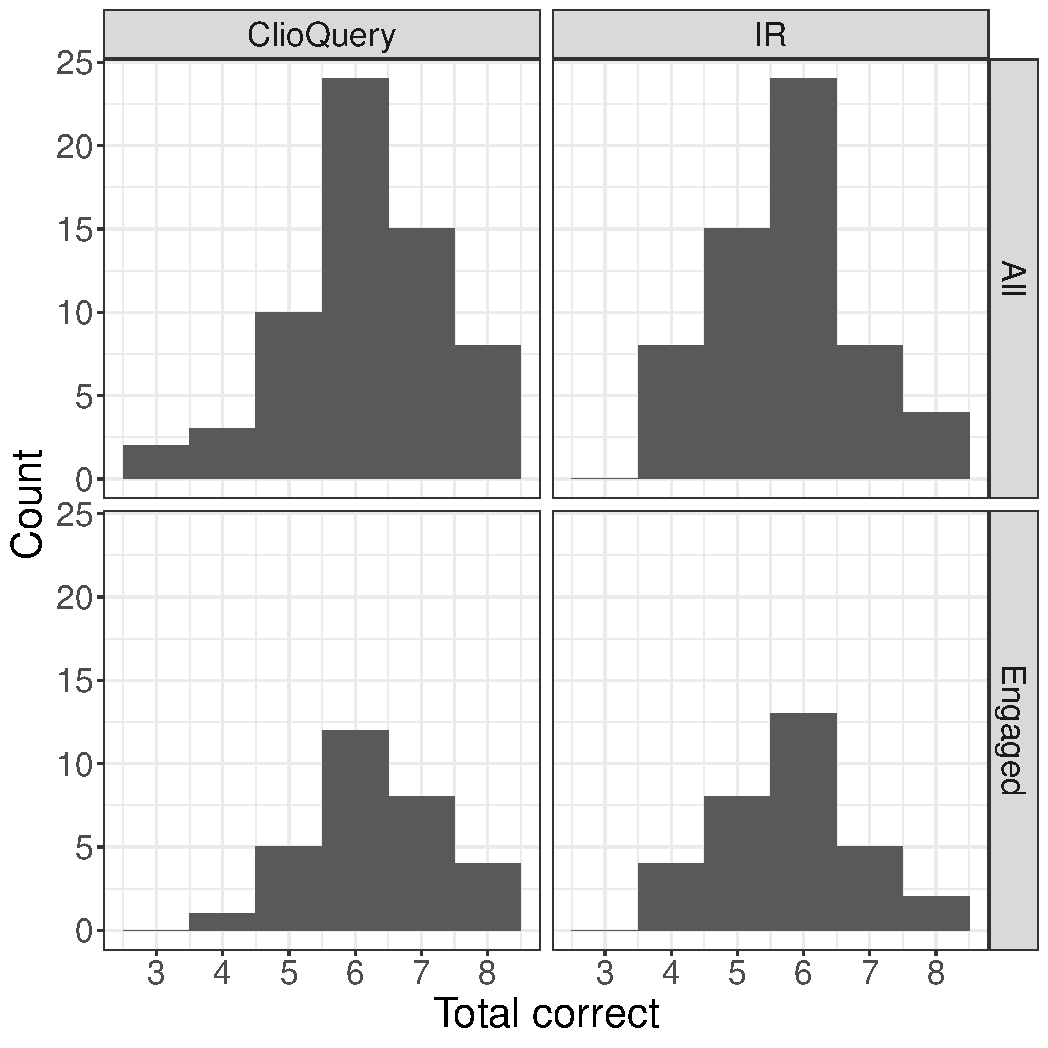
\includegraphics[width=8cm]{figures/faceted_histogram.pdf}
    }\\
    \subfloat{ 
            \begin{tabular}{llccc}
\toprule
 &  & N & Mean correct & Std. Dev.\\
\midrule
\multirow{2}{*}{All*} & ClioQuery & 62 & 6.145 & (1.185)\\
  & IR & 59 & 5.746 & (1.076)\\\midrule
\multirow{2}{*}{Engaged*} & ClioQuery & 30 & 6.300 & (1.022)\\
  & IR & 32 & 5.781 & (1.070)\\
\bottomrule
\end{tabular}
    }
    \caption{Total correct questions by interface, among all participants, and among engaged participants. A star* indicates a significant difference between the means of the \ours~and IR groups.}\label{f:crowdresults}
\end{figure}



\subsection{Results and analysis}

We found that participants assigned to complete the historical reading comprehension task with \ours~averaged more total correct answers than participants assigned to complete the same task with the IR system (Figure \ref{f:crowdresults}). 
Among the \nengaged~engaged participants,
workers in the \ours~group averaged \deltaCQengaged~more correct answers than workers in the IR group (Cohen's $d$=\cohensengaged).\footnote{Computed with v0.8.1 of the \texttt{effsize} package in R.}
\ours's effect was weaker among all participants, where \ours~workers averaged \deltaCQall~more correct answers than IR workers (Cohen's $d$=\cohensALL). 
We hypothesize that this weaker effect may be due to inattention among non-engaged participants, which may have introduced data collection noise.
For instance, participants who did not read task instructions carefully or who failed the pretest may have been more inclined to guess on the Mugabe task.\footnote{The number of workers in each group is not exactly equal. This is common in crowdsourced settings, where some workers may not finish a task. For instance, we used an alert to ask workers attempting to complete our task on a phone rather than a computer to not proceed with the survey.}


\begin{figure}[h]
    \centering
    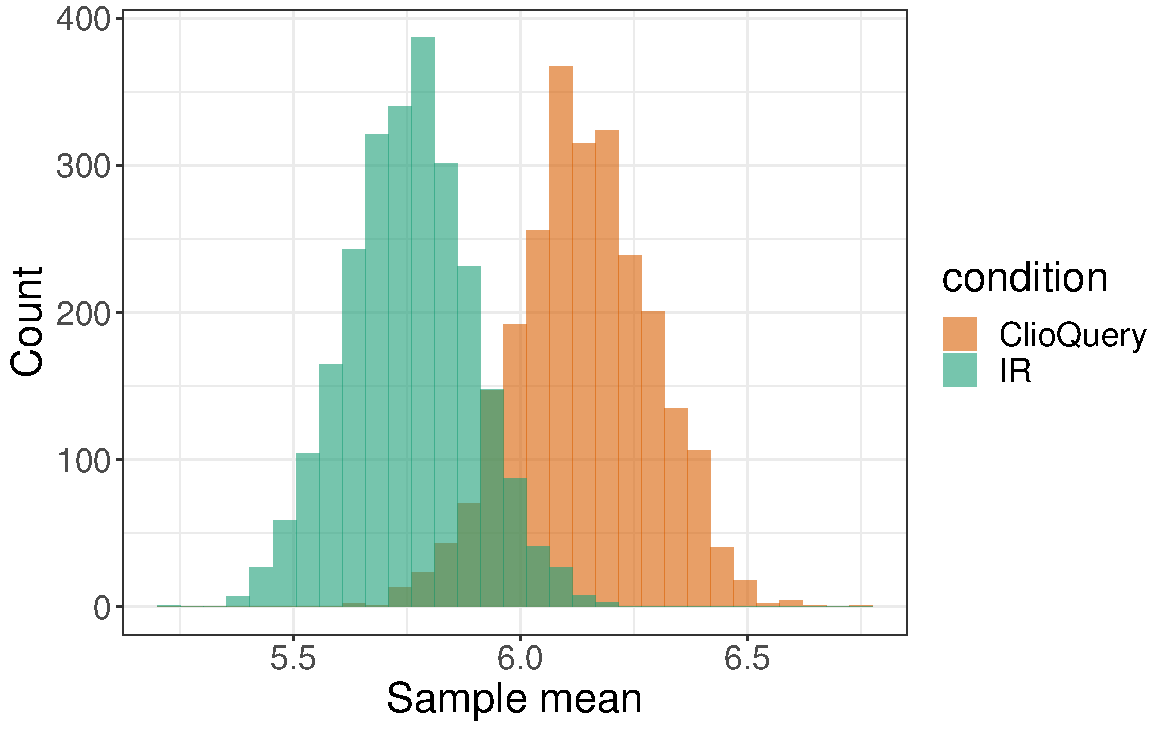
\includegraphics[width=8cm]{figures/bootstrap_means.pdf}
    \caption{Distribution of sample means, across 2500 bootstrap samples of scores from the 59 IR participants, and 2500 separate bootstrap samples of scores from the 62 \ours~participants.}\label{f:samples}
\end{figure}

We tested for possible equality of means using bootstrap hypothesis testing \cite{Efron} (Algorithm 16.2).
Using 100,000 samples, we found that the difference in means among all workers in each condition was significantly different ($p=\pAll$). 
We also found that the difference in means among the subset of engaged workers in each condition was also significant ($p=\pAttentive$). %p values come from turk_processor.py
We show separate bootstrapped distributions of sample means in Figure \ref{f:samples}.




% ./make_qual.sh 
% sec_8_qual.jsonl in public repo has anonymized turker comments
\subsubsection{Qualitative analysis}\label{s:turk_qual}
Our experiment suggested that some properties of the \ours~interface helped participants on the historical reading comprehension task.
To try and gain a better understanding of which exact aspects of \ours~may have been helpful, we reviewed qualitative feedback from the \cqNperfectscore~\ours~participants who achieved a perfect score in reading comprehension.
Each of these participants praised one or more \ours~features in offering qualitative feedback on the system.
\textit{``I liked that I could expand the articles and filter them by the number of times the key word was mentioned,''} one top performer wrote. Said another, \textit{``I liked being able to control the number of mentions so I could determine relevance rather than trust a search engine.''} A third liked that \ours, \textit{``made it easy to see which articles I have already read and which ones I have yet to read.''} One high scorer did note that while in-text highlighting was in general helpful, \textit{``the part of this highlighting that I didn't like is that ... it was hard to gain context without reading the unhighlighted text before or after the highlighted sections.''}

On the other hand, the \irNperfectscore~IR users who got perfect scores offered scattered feedback. One liked how the results did not show \textit{``a bunch of random stuff or products to buy,''} while two others disagreed if the snippets were useful (one praised them, one said they did not help). 
Comments from the final high-scoring IR participant suggested that the IR system offered a realistic baseline. 
\textit{``There wasn't much to like or dislike,''} they said. \textit{``I really didn't find any differences how I would normally do it.''}
